%-----------------------------------------------------------------
\setcounter{currentlevel}{\value{baseSectionLevel}}
\levelstay{Cartesian products}
\label{sec:Cartesian-products}

Combining and factoring sets and functions.

Factor set into product of other sets.

Factor function into 'coordinate' functions:
$f : \Set{X} \rightarrow \Set{Y}_0 \times \Set{Y}_1$
via
$f \left( x \right) = 
\left[ f_0\left( x \right) , f_1\left( x \right) \right]$

Also 'reduce':
$f : \Set{X}_0 \times \Set{X}_1 \rightarrow \Set{Y}$
via 
 $f\left( \left[ x_0, x_1 \right] \right)
= r \left(
\left[ f_0 \left( x_0 \right) , f_1 \left( x_1 \right) \right] 
\right)$,
eg, for linear functions, 
 $f\left( \left[ x_0, x_1 \right] \right)
=  f_0 \left( x_0 \right) + f_1 \left( x_1 \right)$,

%-----------------------------------------------------------------
\setcounter{currentlevel}{\value{baseSectionLevel}-1}
\levelstay{Cartesian product sets}
\label{sec:Cartesian-product-sets}

% \gls{tuple}
A tuple is a fixed length list, which I will write, for example,
$[a \, b \, c]$, in a Clojure-like syntax,
or sometimes as $a \times b \times c$.

% \gls{cartesian-product}
The cartesian product set 
$\Set{A} \times \Set{B} =
\SetSpec{[a \, b] }{ a \in \Set{A} \text{ and } b \in \Set{B} }$.

Extending this notation beyond two terms,
$\Set{A} \times \Set{B} \times \Set{C}$,
introduces ambiguity typically ignored in mathematics literature,
using the implied natural identity mentioned above.
Strictly speaking,
\begin{itemize}
  \item $\Set{A} \times \Set{B} \times \Set{C} = 
  \SetSpec{[a \, b \, c] }{ \ldots }$
  \item $\Set{A} \times (\Set{B} \times \Set{C}) = 
  \SetSpec{[a \, [b \,c]] }{ \ldots }$
  \item $(\Set{A} \times \Set{B}) \times \Set{C} = 
  \SetSpec{[[a \, b] \, c]] }{ \ldots }$
\end{itemize}
are 3 distinct sets.

%-----------------------------------------------------------------
\setcounter{currentlevel}{\value{baseSectionLevel}-1}
\levelstay{Generalized tuples}
\label{sec:Generalized-tuples}

Tuples as functions from index set to set elements.

'Subspace' corresponds to subset of index set.

Canonical projections and embeddings.

Generalized coordinates.

%-----------------------------------------------------------------
\setcounter{currentlevel}{\value{baseSectionLevel}-1}
\levelstay{Cartesion product functions}
\label{sec:Cartesion-product-functions}

Aka \textit{coordinate functions}.

Suppose $f : \Set{X} \rightarrow \Set{Y}_0 \times \Set{Y}_1$,
and $f \left( x \right) = \left[ y_0 ,y_1 \right]$
Then we can write $f = f_0 \times f_1$ where
$f_0 \left( x \right) = y_0 $
and
$f_1 \left( x \right) = y_1 $.

\textbf{TODO:} $f$ corresponds to a functional relation on 
$\Set{X} \times \left( \Set{Y}_0 \times \Set{Y}-1 \right)$).
Does this imply functional relations $f_i$ on
$\Set{X} \times \Set{Y}_i$?
How about $f_i = e_i \circ f$,
where $e_i : \times_j \Set{X}_j  \rightarrow \Set{X}_i$ by
$e_i \left( [x_0, x_1, \ldots , x_{n-1} \right) = x_i$ 

%-----------------------------------------------------------------
\setcounter{currentlevel}{\value{baseSectionLevel}-1}
\levelstay{Implementation}

%-----------------------------------------------------------------
\setcounter{currentlevel}{\value{baseSectionLevel}-2}
\levelstay{Java}
\lstset{language=Java}

Java provides an interface \lstinline|java.util.Set| intended for
possibly mutable, finite sets (\autoref{java.util.Set:general},
 \autoref{java.util.Set:countable}, 
 \autoref{java.util.Set:finite}, 
 and
\autoref{java.util.Set:optional}).

%-----------------------------------------------------------------
\begin{lstlisting}[
 caption={[\texttt{java.util.Set} general]\texttt{java.util.Set} 
 operations applicable to any set.}, 
 label=java.util.Set:general]
boolean contains (Object o) //$ \; o \in \Set{S}$
boolean containsAll (Collection c) //$\;\Set{C}\subseteq\Set{S}$ 
boolean isEmpty () //$ \; \Set{S} = \varnothing $
boolean equals (Object o) //$\; \Set{S} = \Set{O} $
\end{lstlisting}
%-----------------------------------------------------------------
\begin{lstlisting}[
 caption={[\texttt{java.util.Set} countable]\texttt{java.util.Set} 
 operations requiring countable sets. Note, however, that 
 iterators that never end will cause havoc with almost all Java
 code}, 
 label=java.util.Set:countable]
Iterator iterator ()
Spliterator spliterator ()
\end{lstlisting}
%-----------------------------------------------------------------
\begin{lstlisting}[
 caption={[\texttt{java.util.Set} finite]\texttt{java.util.Set} 
 operations requiring finite sets. Note that changing to
 \texttt{size()} to be Object valued would enable representing sets
 of arbitrary cardinality.}, 
 label=java.util.Set:finite] 
int size () 
Object[] toArray ()
Object[] toArray (Object[] a)
\end{lstlisting}
%-----------------------------------------------------------------
\begin{lstlisting}[
 caption={[\texttt{java.util.Set}]\texttt{java.util.Set} optional
 operations, requiring mutable sets.}, 
 label=java.util.Set:optional,]
boolean add(E e) //$\; \Set{S} \leftarrow \Set{S} \cup \{e\} $
boolean addAll(Collection c) //$\;\Set{S}\leftarrow\Set{S}\cup\Set{C}$ 
void  clear() //$\; \Set{S} \leftarrow \varnothing $ 
boolean remove (Object o) //$\;\Set{S}\leftarrow\Set{S}\setminus\{e\}$
boolean removeAll (Collection c) //$\;\Set{S}\leftarrow\Set{S}\setminus\Set{C}$ 
boolean retainAll (Collection c) //$\;\Set{S}\leftarrow\Set{S}\cap\Set{C}$
\end{lstlisting}
%-----------------------------------------------------------------

More Java set classes? Guava or Apache Commons?
Set operations, union, cartesian products, \ldots.

%-----------------------------------------------------------------
\setcounter{currentlevel}{\value{baseSectionLevel}-2}
\levelstay{Clojure}
\lstset{language=Clojure}

Idiomatic Clojure sets are immutable, although it provides easy
access to any mutable or immutable Java implementation of
\lstinline|java.util.Set|.

Clojure provides an (unfortunate) literal syntax for finite
enumerated sets: 
\lstinline|#{0 1 2}|, and 4 ways to create sets:
\begin{description}
\item[\texttt{hash-set}] A function equivalent to the
literal syntax \lstinline|#{}|
\item[\texttt{sorted-set}/\texttt{sorted-set-by}] Returns
sets that iterate over their elements in their natural order (in the
order of the supplied comparator). Like Java sorted collections,
can't handle partial orderings.
\item[\texttt{set}] Coerce any collection into a set.
\item[\texttt{into}] A general way to coerce any collection
into another type.
\end{description}

Idiomatic Clojure provides an informally specified functional
'API' for finite sets. Most of these functions do will something
for all Clojure collections, not always what you would expect:
\begin{lstlisting}[
 caption={Clojure set 'API'}, 
 label=Clojure:set-API,]
(contains? s x) ;;  $x \in \Set{S}$.
(empty? s) ;; $\Set{S} = \varnothing$
(count s) ;; $\text{cardinality}(\Set{S})$
(conj s x) ;; $\Set{S} \cup \{x\}$
(disj s x) ;; $\Set{S} \setminus \{x\}$
(clojure.set/intersection s0 s1 s2 $\ldots$) ;; $\Set{S}_0 \cap \Set{S}_1 \cap \Set{S}_2 \cap \ldots$ 
(clojure.set/union s0 s1 s2 $\ldots$) ;; $\Set{S}_0 \cup \Set{S}_1 \cup \Set{S}_2 \cup \ldots$ 
(clojure.set/difference s0 s1 s2 $\ldots$) ;; $\Set{S}_0 \setminus (\Set{S}_1 \cup \Set{S}_2 \cup \ldots)$
\end{lstlisting}

Confusion with dictionary 'API':
 \lstinline|(s x)| and \lstinline|(get s x)| are similar to
 \lstinline|(contains? s x)| except \lstinline|(contains? s x)| returns
 \lstinline|true| or \lstinline|false|, while the other two return
 \lstinline|x| if \lstinline|x| is in \lstinline|s| \lstinline|nil| otherwise.
The behavior of \lstinline|(s x)| and \lstinline|(get s x)| reflect an
incomplete/inconsistent API treating Clojure collections as
dictionaries (key-value pairs), modeling sets as dictionaries
where the key and value are constrained to be the same.
However, other functions designed for dictionaries (eg
\lstinline|keys|) don't work for sets.
 
%-----------------------------------------------------------------
\setcounter{currentlevel}{\value{baseSectionLevel}-2}
\levelstay{Les Elemens}

Set interface:

% \begin{lstlisting}[
% caption={[checksum namespace]Checksum and related functions via
% Java calls}, label=checksum-namespace,]
% (set! *warn-on-reflection* true)
% (set! *unchecked-math* :warn-on-boxed)
% (ns ^{:doc "compute a file checksum."}
%   
%   curate.scripts.checksum
%   
%   (:require [clojure.java.io :as io])
%   (:use [clojure.set :only [difference]])
%   (:gen-class))
% ;;-----------------------------------------------------------------
% (defn checksum [file]
%   (let [input (java.io.FileInputStream. file)
%         digest (java.security.MessageDigest/getInstance "MD5")
%         stream (java.security.DigestInputStream. input digest)
%         bufsize (* 1024 1024)
%         buf (byte-array bufsize)]
% 
%   (while (not= -1 (.read stream buf 0 bufsize)))
%   (apply str (map (partial format "%02x") (.digest digest)))))
% 
% (defn list-dir [dir]
%   (remove #(.isDirectory %)
%           (file-seq (java.io.File. dir))))
% 
% (defn find-dupes [root]
%   (let [files (list-dir root)]
%     (let [summed (zipmap (pmap #(checksum %) files) files)]
%       (difference
%        (into #{} files)
%        (into #{} (vals summed))))))
% 
% (defn remove-dupes [files]
%   (prn "Duplicates files to be removed:")
%   (doseq [f files] (prn (.toString f)))
%   (prn "Delete files? [y/n]:")
%   (if-let [choice (= (read-line) "y")]
%     (doseq [f files] (.delete f))))
% 
% (defn -main [& args]
%   (if (empty? args)
%     (println "Enter a root directory")
%     (remove-dupes (find-dupes (first args))))
%   (System/exit 0))
% \end{lstlisting}
% 
% \lstinputlisting[
% float=htbp,
% caption={[checksum function]Compute a checksum for a file thru Java},
% label=checksum,
% firstline=11,lastline=18]{listings/checksum.clj}
 
%-----------------------------------------------------------------
\setcounter{currentlevel}{\value{baseSectionLevel}-1}
\levelstay{Examples}
 
% \begin{minipage}{\linewidth}
% \begin{lstlisting}[
% caption={[FileTypeFilter]A file .suffix filter},
% label=FileTypeFilter]
% package img;
% 
% public final class FileTypeFilter 
%   implements java.io.FilenameFilter {
% 
%   private final String _suffix;
% 
%   public final boolean accept (final java.io.File dir,
%                                final String name) {
%     return name.toLowerCase().endsWith(_suffix); }
% 
%   public FileTypeFilter (final String suffix) {
%     super();
%     _suffix = suffix.toLowerCase(); } }
% \end{lstlisting}
% \end{minipage}
% 
% \index{Sets|)}
% 
% \begin{figure}[htbp]
% \centering
% 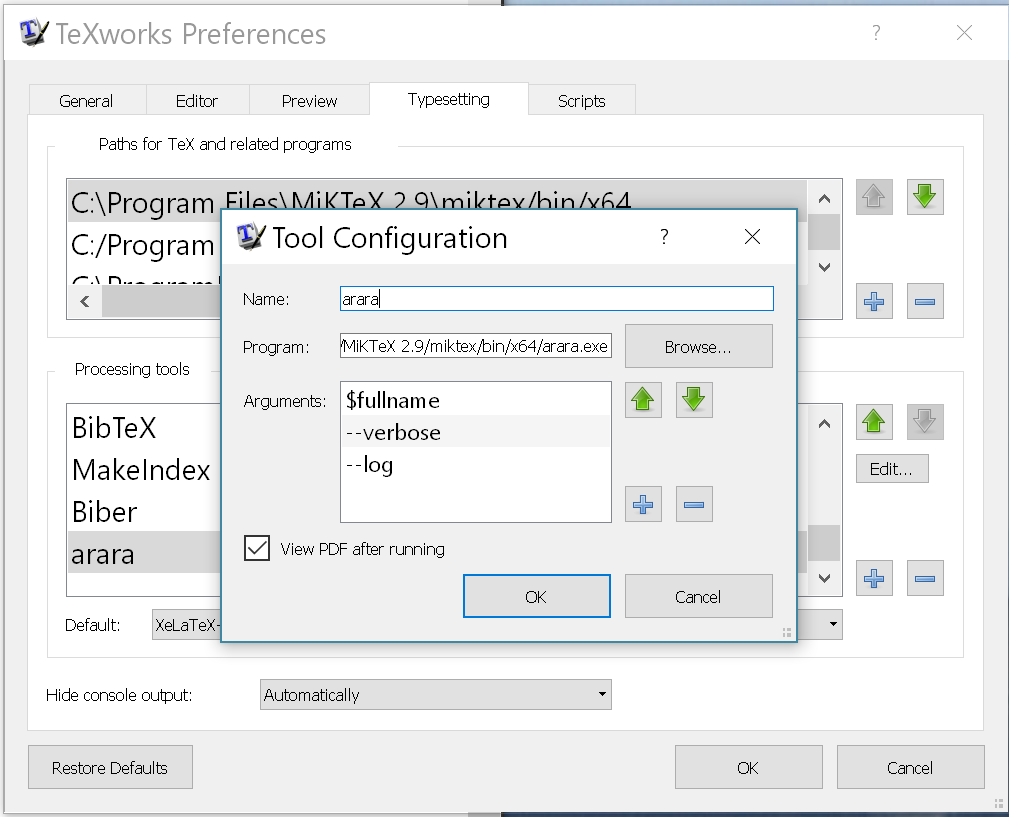
\includegraphics[scale=0.7]{figs/arara.png}
% \caption{Configuring {\TeX}works for \texttt{arara}.}
% \end{figure}
